%---------------
%╔═╗╔═╗╔╦╗╦ ╦╔═╗
%╚═╗║╣  ║ ║ ║╠═╝
%╚═╝╚═╝ ╩ ╚═╝╩
%---------------

% language setup
\newcommand{\docLanguage}{ngerman}
%\newcommand{\docLanguage}{english}

% DOCUMENT SETUP
\documentclass[12pt, oneside, a4paper, \docLanguage]{report}
\usepackage[left=3cm,
			right=2.5cm,
			top=2.5cm,
			bottom=2.5cm,
			includehead,
			includefoot]{geometry}

% line spacing
\usepackage{setspace}
\setstretch{1,25} % 15/12 --> 1.25

% encoding setup
% T1 font encoding for languages that use a latin alphabet
\usepackage[T1]{fontenc}

% enhanced input encoding handling - utf8 for äÄüÜöÖß...
\usepackage[utf8]{inputenc}

%de­fines Adobe Times Ro­man as de­fault text font
\usepackage{mathptmx}
\usepackage{times} % needed for acronym package

%PDF linking package
\usepackage[hidelinks]{hyperref}


% Language Setup
\usepackage[\docLanguage]{babel}
% after babel - set chapter string
\AtBeginDocument{\renewcommand{\chaptername}{}}

% language specific bibliography style
\usepackage[numbers, square]{natbib}
%\setcitestyle{square,aysep={},yysep={;}}
\usepackage{babelbib}
% bliographystyle setup
% babel specific: babplain, babplai3, babalpha, babunsrt, bababbrv, bababbr3
\bibliographystyle{babunsrt}


% enumeration
\usepackage{enumitem}
% tabular extension tabularx
\usepackage{tabularx}

% math packages
\usepackage{amsmath}
\usepackage{nicefrac}
\usepackage{amsthm}
\usepackage{amsbsy}
\usepackage{amssymb}
\usepackage{amsfonts}
%\usepackage{MnSymbol}


%special characters
\usepackage{amssymb}
\usepackage{upgreek,textgreek}

% acronym package
\usepackage[printonlyused, footnote]{acronym}

% breakable text in \seqsplit{}
\usepackage{seqsplit}

% \textmu
\usepackage{textcomp}

% package provides a way to compile sections of a document using the same preamble as the main document
\usepackage{subfiles}

% driver-independent color extension - used by listings,tabularx
\usepackage[usenames,dvipsnames,table,xcdraw]{xcolor}

% -- SYNTAX HIGHLIGHTING --
\usepackage{listings}
%% bash command line Syntax Highlighting
\lstdefinestyle{BASH_CMD}{ 
  columns=fullflexible,            % copy pasteable listings
  language=bash,
  basicstyle=\small\sffamily,
  basicstyle   = \small \ttfamily,
  keywordstyle = [1]\small \ttfamily,
  keywordstyle = [2]\small \ttfamily,
  commentstyle = \small \ttfamily,
  numbers=none,
  captionpos=b, 
  breaklines=true,
  numberstyle=\tiny,
  numbersep=3pt,
  frame=tlrb,
  columns=fullflexible,
  backgroundcolor=\color{white!20},
  linewidth=\linewidth,
  literate=                        % replace in code
     {Ö}{{\"O}}1 
     {Ä}{{\"A}}1 
     {Ü}{{\"U}}1 
     {ß}{{\ss}}2 
     {ü}{{\"u}}1 
     {ä}{{\"a}}1 
     {ö}{{\"o}}1 
     {â}{{\^{a}}}1 
     {Â}{{\^{A}}}1 
     {ç}{{\c{c}}}1 
     {Ç}{{\c{C}}}1 
     {ğ}{{\u{g}}}1 
     {Ğ}{{\u{G}}}1 
     {ı}{{\i}}1 
     {İ}{{\.{I}}}1 
     {ş}{{\c{s}}}1 
     {Ş}{{\c{S}}}1 
}
 % adds style BASH_CMD
%% Matlab Syntax Highlighting
\colorlet{keyword}{blue!100!black!80}
\colorlet{STD}{Lavender}
\colorlet{comment}{green!90!black!90}
\definecolor{mygreen}{rgb}{0,0.6,0}
\definecolor{mygray}{rgb}{0.5,0.5,0.5}
\definecolor{mymauve}{rgb}{0.58,0,0.82}


\lstdefinestyle{BASH_SCRIPT}{ 
  language     = bash,
  basicstyle   = \footnotesize \ttfamily,
  keywordstyle = [1]\color{keyword}\bfseries,
  keywordstyle = [2]\color{STD}\bfseries,
  commentstyle = \color{mygreen}\itshape,
  backgroundcolor=\color{white},   % choose the background color; you must add \usepackage{color} 
  columns=fullflexible,            % copy pasteable listings
                                   % or \usepackage{xcolor}
  basicstyle=\footnotesize,        % the size of the fonts that are used for the code
  breakatwhitespace=false,         % sets if automatic breaks should only happen at whitespace
  breaklines=true,                 % sets automatic line breaking
  captionpos=b,                    % sets the caption-position to bottom
  extendedchars=true,              % lets you use non-ASCII characters; for 8-bits encodings only,
                                   % does not work with UTF-8
  frame=single,                    % adds a frame around the code
  keepspaces=true,                 % keeps spaces in text, useful for keeping indentation of code
                                   % (possibly needs columns=flexible)
  numbers=left,                    % where to put the line-numbers; possible values are 
                                   % (none, left, right)
  numbersep=5pt,                   % how far the line-numbers are from the code
  numberstyle=\tiny\color{mygray}, % the style that is used for the line-numbers
  rulecolor=\color{black},         % if not set, the frame-color may be changed on line-breaks
                                   % within not-black text (e.g. comments (green here))
  showspaces=false,                % show spaces everywhere adding particular underscores; it
  	                               % overrides 'showstringspaces'
  showstringspaces=false,          % underline spaces within strings only
  showtabs=false,                  % show tabs within strings adding particular underscores
  stepnumber=1,                    % the step between two line-numbers. If it's 1, each line 
                                   % will be numbered
  stringstyle=\color{mymauve},     % string literal style
  tabsize=2,                       % sets default tabsize to 2 spaces
  title=\lstname,                  % set title name
  literate=                        % replace in code
     {Ö}{{\"O}}1 
     {Ä}{{\"A}}1 
     {Ü}{{\"U}}1 
     {ß}{{\ss}}2 
     {ü}{{\"u}}1 
     {ä}{{\"a}}1 
     {ö}{{\"o}}1 
     {â}{{\^{a}}}1 
     {Â}{{\^{A}}}1 
     {ç}{{\c{c}}}1 
     {Ç}{{\c{C}}}1 
     {ğ}{{\u{g}}}1 
     {Ğ}{{\u{G}}}1 
     {ı}{{\i}}1 
     {İ}{{\.{I}}}1 
     {ş}{{\c{s}}}1 
     {Ş}{{\c{S}}}1 
} % adds style BASH_SCRIPT
% Matlab Syntax Highlighting
\colorlet{keyword}{blue!100!black!80}
\colorlet{STD}{red}
\colorlet{comment}{green!90!black!90}
\definecolor{mygreen}{rgb}{0,0.6,0}
\definecolor{mygray}{rgb}{0.5,0.5,0.5}
\definecolor{mymauve}{rgb}{0.58,0,0.82}


\lstdefinestyle{LATEX}{ 
  language     = [LaTeX]{TeX},
  basicstyle   = \footnotesize \ttfamily,
  keywordstyle = [1]\color{keyword}\bfseries,
  keywordstyle = [2]\color{comment}\bfseries,
  commentstyle = \color{mygray}\itshape,
  %backgroundcolor=\color{white},   % choose the background color; you must add \usepackage{color} 
                                   % or \usepackage{xcolor}
  basicstyle=\footnotesize,        		   % the size of the fonts that are used for the code
  breakatwhitespace=false,         % sets if automatic breaks should only happen at whitespace
  columns=fullflexible,            % copy pasteable listings
  breaklines=true,                 % sets automatic line breaking
  captionpos=c,                    % sets the caption-position to bottom
  extendedchars=true,              % lets you use non-ASCII characters; for 8-bits encodings only,
                                   % does not work with UTF-8
  frame=single,                    % adds a frame around the code
  keepspaces=true,                 % keeps spaces in text, useful for keeping indentation of code
                                   % (possibly needs columns=flexible)
  numbers=left,                    % where to put the line-numbers; possible values are 
                                   % (none, left, right)
  numbersep=4pt,                   % how far the line-numbers are from the code
  numberstyle=\tiny\color{mygray}, % the style that is used for the line-numbers
  rulecolor=\color{black},         % if not set, the frame-color may be changed on line-breaks
                                   % within not-black text (e.g. comments (green here))
  showspaces=false,                % show spaces everywhere adding particular underscores; it
  	                               % overrides 'showstringspaces'
  showstringspaces=false,          % underline spaces within strings only
  showtabs=false,                  % show tabs within strings adding particular underscores
  stepnumber=1,                    % the step between two line-numbers. If it's 1, each line 
                                   % will be numbered
  stringstyle=\color{mymauve},     % string literal style
  tabsize=2,                       % sets default tabsize to 2 spaces
  title=\lstname,                  % set title name
  literate=                        % replace in code
     {Ö}{{\"O}}1 
     {Ä}{{\"A}}1 
     {Ü}{{\"U}}1 
     {ß}{{\ss}}2 
     {ü}{{\"u}}1 
     {ä}{{\"a}}1 
     {ö}{{\"o}}1 
     {â}{{\^{a}}}1 
     {Â}{{\^{A}}}1 
     {ç}{{\c{c}}}1 
     {Ç}{{\c{C}}}1 
     {ğ}{{\u{g}}}1 
     {Ğ}{{\u{G}}}1 
     {ı}{{\i}}1 
     {İ}{{\.{I}}}1 
     {ş}{{\c{s}}}1 
     {Ş}{{\c{S}}}1 
} % adds style LATEX
%% Matlab Syntax Highlighting
\colorlet{keyword}{blue!100!black!80}
\colorlet{STD}{Lavender}
\colorlet{comment}{green!90!black!90}
\definecolor{mygreen}{rgb}{0,0.6,0}
\definecolor{mygray}{rgb}{0.5,0.5,0.5}
\definecolor{mymauve}{rgb}{0.58,0,0.82}


\lstdefinestyle{MATLAB}{ 
  language     = Matlab,
  basicstyle   = \footnotesize \ttfamily,
  keywordstyle = [1]\color{keyword}\bfseries,
  keywordstyle = [2]\color{STD}\bfseries,
  commentstyle = \color{mygreen}\itshape,
  backgroundcolor=\color{white},   % choose the background color; you must add \usepackage{color} 
                                   % or \usepackage{xcolor}
  basicstyle=\footnotesize,        % the size of the fonts that are used for the code
  breakatwhitespace=false,         % sets if automatic breaks should only happen at whitespace
  columns=fullflexible,            % copy pasteable listings
  breaklines=false,                % sets automatic line breaking
  captionpos=c,                    % sets the caption-position to bottom
  extendedchars=true,              % lets you use non-ASCII characters; for 8-bits encodings only,
                                   % does not work with UTF-8
  frame=single,                    % adds a frame around the code
  keepspaces=true,                 % keeps spaces in text, useful for keeping indentation of code
                                   % (possibly needs columns=flexible)
  numbers=left,                    % where to put the line-numbers; possible values are 
                                   % (none, left, right)
  numbersep=5pt,                   % how far the line-numbers are from the code
  numberstyle=\tiny\color{mygray}, % the style that is used for the line-numbers
  rulecolor=\color{black},         % if not set, the frame-color may be changed on line-breaks
                                   % within not-black text (e.g. comments (green here))
  showspaces=false,                % show spaces everywhere adding particular underscores; it
  	                               % overrides 'showstringspaces'
  showstringspaces=false,          % underline spaces within strings only
  showtabs=false,                  % show tabs within strings adding particular underscores
  stepnumber=1,                    % the step between two line-numbers. If it's 1, each line 
                                   % will be numbered
  stringstyle=\color{mymauve},     % string literal style
  tabsize=2,                       % sets default tabsize to 2 spaces
  title=\lstname,                  % set title name
  literate=                        % replace in code
     {Ö}{{\"O}}1 
     {Ä}{{\"A}}1 
     {Ü}{{\"U}}1 
     {ß}{{\ss}}2 
     {ü}{{\"u}}1 
     {ä}{{\"a}}1 
     {ö}{{\"o}}1 
     {â}{{\^{a}}}1 
     {Â}{{\^{A}}}1 
     {ç}{{\c{c}}}1 
     {Ç}{{\c{C}}}1 
     {ğ}{{\u{g}}}1 
     {Ğ}{{\u{G}}}1 
     {ı}{{\i}}1 
     {İ}{{\.{I}}}1 
     {ş}{{\c{s}}}1 
     {Ş}{{\c{S}}}1 
} % adds style MATLAB
% Matlab Syntax Highlighting
\colorlet{keyword}{blue!100!black!80}
\colorlet{STD}{Lavender}
\colorlet{comment}{green!90!black!90}
\definecolor{mygreen}{rgb}{0,0.6,0}
\definecolor{mygray}{rgb}{0.5,0.5,0.5}
\definecolor{mymauve}{rgb}{0.58,0,0.82}


\lstdefinestyle{PYTHON}{ 
  language     = Python,
  basicstyle   = \footnotesize \ttfamily,
  keywordstyle = [1]\color{keyword}\bfseries,
  keywordstyle = [2]\color{STD}\bfseries,
  commentstyle = \color{mygreen}\itshape,
  backgroundcolor=\color{white},   % choose the background color; you must add \usepackage{color} 
                                   % or \usepackage{xcolor}
  basicstyle=\footnotesize,        % the size of the fonts that are used for the code
  columns=fullflexible,            % copy pasteable listings
  breakatwhitespace=false,         % sets if automatic breaks should only happen at whitespace
  breaklines=false,                % sets automatic line breaking
  captionpos=c,                    % sets the caption-position to bottom
  extendedchars=true,              % lets you use non-ASCII characters; for 8-bits encodings only,
                                   % does not work with UTF-8
  frame=single,                    % adds a frame around the code
  keepspaces=true,                 % keeps spaces in text, useful for keeping indentation of code
                                   % (possibly needs columns=flexible)
  numbers=left,                    % where to put the line-numbers; possible values are 
                                   % (none, left, right)
  numbersep=5pt,                   % how far the line-numbers are from the code
  numberstyle=\tiny\color{mygray}, % the style that is used for the line-numbers
  rulecolor=\color{black},         % if not set, the frame-color may be changed on line-breaks
                                   % within not-black text (e.g. comments (green here))
  showspaces=false,                % show spaces everywhere adding particular underscores; it
  	                               % overrides 'showstringspaces'
  showstringspaces=false,          % underline spaces within strings only
  showtabs=false,                  % show tabs within strings adding particular underscores
  stepnumber=1,                    % the step between two line-numbers. If it's 1, each line 
                                   % will be numbered
  stringstyle=\color{mymauve},     % string literal style
  tabsize=2,                       % sets default tabsize to 2 spaces
  title=\lstname,                  % set title name
  literate=                        % replace in code
     {Ö}{{\"O}}1 
     {Ä}{{\"A}}1 
     {Ü}{{\"U}}1 
     {ß}{{\ss}}2 
     {ü}{{\"u}}1 
     {ä}{{\"a}}1 
     {ö}{{\"o}}1 
     {â}{{\^{a}}}1 
     {Â}{{\^{A}}}1 
     {ç}{{\c{c}}}1 
     {Ç}{{\c{C}}}1 
     {ğ}{{\u{g}}}1 
     {Ğ}{{\u{G}}}1 
     {ı}{{\i}}1 
     {İ}{{\.{I}}}1 
     {ş}{{\c{s}}}1 
     {Ş}{{\c{S}}}1 
} % adds style PYTHON
%% Matlab Syntax Highlighting
\colorlet{keyword}{blue!100!black!80}
\colorlet{STD}{Lavender}
\colorlet{comment}{green!90!black!90}
\definecolor{mygreen}{rgb}{0,0.6,0}
\definecolor{mygray}{rgb}{0.5,0.5,0.5}
\definecolor{mymauve}{rgb}{0.58,0,0.82}


\lstdefinestyle{CPP}{ 
  language     = C++,
  basicstyle   = \footnotesize \ttfamily,
  keywordstyle = [1]\color{keyword}\bfseries,
  keywordstyle = [2]\color{STD}\bfseries,
  commentstyle = \color{mygreen}\itshape,
  backgroundcolor=\color{white},   % choose the background color; you must add \usepackage{color} 
                                   % or \usepackage{xcolor}
  columns=fullflexible,            % copy pasteable listings
  basicstyle=\footnotesize,        % the size of the fonts that are used for the code
  breakatwhitespace=false,         % sets if automatic breaks should only happen at whitespace
  breaklines=false,                % sets automatic line breaking
  captionpos=c,                    % sets the caption-position to bottom
  extendedchars=true,              % lets you use non-ASCII characters; for 8-bits encodings only,
                                   % does not work with UTF-8
  frame=single,                    % adds a frame around the code
  keepspaces=true,                 % keeps spaces in text, useful for keeping indentation of code
                                   % (possibly needs columns=flexible)
  numbers=left,                    % where to put the line-numbers; possible values are 
                                   % (none, left, right)
  numbersep=5pt,                   % how far the line-numbers are from the code
  numberstyle=\tiny\color{mygray}, % the style that is used for the line-numbers
  rulecolor=\color{black},         % if not set, the frame-color may be changed on line-breaks
                                   % within not-black text (e.g. comments (green here))
  showspaces=false,                % show spaces everywhere adding particular underscores; it
  	                               % overrides 'showstringspaces'
  showstringspaces=false,          % underline spaces within strings only
  showtabs=false,                  % show tabs within strings adding particular underscores
  stepnumber=1,                    % the step between two line-numbers. If it's 1, each line 
                                   % will be numbered
  stringstyle=\color{mymauve},     % string literal style
  tabsize=2,                       % sets default tabsize to 2 spaces
  title=\lstname,                  % set title name
  literate=                        % replace in code
     {Ö}{{\"O}}1 
     {Ä}{{\"A}}1 
     {Ü}{{\"U}}1 
     {ß}{{\ss}}2 
     {ü}{{\"u}}1 
     {ä}{{\"a}}1 
     {ö}{{\"o}}1 
     {â}{{\^{a}}}1 
     {Â}{{\^{A}}}1 
     {ç}{{\c{c}}}1 
     {Ç}{{\c{C}}}1 
     {ğ}{{\u{g}}}1 
     {Ğ}{{\u{G}}}1 
     {ı}{{\i}}1 
     {İ}{{\.{I}}}1 
     {ş}{{\c{s}}}1 
     {Ş}{{\c{S}}}1 
} % adds style CPP
%% Matlab Syntax Highlighting
\colorlet{keyword}{blue!100!black!80}
\colorlet{STD}{Lavender}
\colorlet{comment}{green!90!black!90}
\definecolor{mygreen}{rgb}{0,0.6,0}
\definecolor{mygray}{rgb}{0.5,0.5,0.5}
\definecolor{mymauve}{rgb}{0.58,0,0.82}


\lstdefinestyle{C}{ 
  language     = C,
  basicstyle   = \footnotesize \ttfamily,
  keywordstyle = [1]\color{keyword}\bfseries,
  keywordstyle = [2]\color{STD}\bfseries,
  commentstyle = \color{mygreen}\itshape,
  backgroundcolor=\color{white},   % choose the background color; you must add \usepackage{color} 
  columns=fullflexible,            % copy pasteable listings
                                   % or \usepackage{xcolor}
  basicstyle=\footnotesize,        % the size of the fonts that are used for the code
  breakatwhitespace=false,         % sets if automatic breaks should only happen at whitespace
  breaklines=false,                % sets automatic line breaking
  captionpos=c,                    % sets the caption-position to bottom
  extendedchars=true,              % lets you use non-ASCII characters; for 8-bits encodings only,
                                   % does not work with UTF-8
  frame=single,                    % adds a frame around the code
  keepspaces=true,                 % keeps spaces in text, useful for keeping indentation of code
                                   % (possibly needs columns=flexible)
  numbers=left,                    % where to put the line-numbers; possible values are 
                                   % (none, left, right)
  numbersep=5pt,                   % how far the line-numbers are from the code
  numberstyle=\tiny\color{mygray}, % the style that is used for the line-numbers
  rulecolor=\color{black},         % if not set, the frame-color may be changed on line-breaks
                                   % within not-black text (e.g. comments (green here))
  showspaces=false,                % show spaces everywhere adding particular underscores; it
  	                               % overrides 'showstringspaces'
  showstringspaces=false,          % underline spaces within strings only
  showtabs=false,                  % show tabs within strings adding particular underscores
  stepnumber=1,                    % the step between two line-numbers. If it's 1, each line 
                                   % will be numbered
  stringstyle=\color{mymauve},     % string literal style
  tabsize=2,                       % sets default tabsize to 2 spaces
  title=\lstname,                  % set title name
  literate=                        % replace in code
     {Ö}{{\"O}}1 
     {Ä}{{\"A}}1 
     {Ü}{{\"U}}1 
     {ß}{{\ss}}2 
     {ü}{{\"u}}1 
     {ä}{{\"a}}1 
     {ö}{{\"o}}1 
     {â}{{\^{a}}}1 
     {Â}{{\^{A}}}1 
     {ç}{{\c{c}}}1 
     {Ç}{{\c{C}}}1 
     {ğ}{{\u{g}}}1 
     {Ğ}{{\u{G}}}1 
     {ı}{{\i}}1 
     {İ}{{\.{I}}}1 
     {ş}{{\c{s}}}1 
     {Ş}{{\c{S}}}1 
} % adds style C
%% JSON Syntax Highlighting
\colorlet{keyword}{blue!100!black!80}
\colorlet{STD}{Lavender}
\colorlet{comment}{green!90!black!90}
\definecolor{mygreen}{rgb}{0,0.6,0}
\definecolor{mygray}{rgb}{0.5,0.5,0.5}
\definecolor{mymauve}{rgb}{0.58,0,0.82}

\newcommand\JSONnumbervaluestyle{\color{blue}}
\newcommand\JSONstringvaluestyle{\color{red}}

\newif\ifcolonfoundonthisline

\makeatletter

\lstdefinelanguage{json}
{
  showstringspaces    = false,
  keywords            = {false,true},
  alsoletter          = 0123456789.,
  morestring          = [s]{"}{"},
  morestring          = [s]{'}{'},
  stringstyle         = \ifcolonfoundonthisline\JSONstringvaluestyle\fi,
  MoreSelectCharTable =%
    \lst@DefSaveDef{`:}\colon@json{\processColon@json},
  basicstyle          = \ttfamily,
  keywordstyle        = \ttfamily\bfseries,
}

% flip the switch if a colon is found in Pmode
\newcommand\processColon@json{
  \colon@json%
  \ifnum\lst@mode=\lst@Pmode%
    \global\colonfoundonthislinetrue%
  \fi
}

\lst@AddToHook{Output}{%
  \ifcolonfoundonthisline%
    \ifnum\lst@mode=\lst@Pmode%
      \def\lst@thestyle{\JSONnumbervaluestyle}%
    \fi
  \fi
  %override by keyword style if a keyword is detected!
  \lsthk@DetectKeywords% 
}

% reset the switch at the end of line
\lst@AddToHook{EOL}%
  {\global\colonfoundonthislinefalse}

\makeatother



\lstdefinestyle{JSON}{ 
  language     = json,
  basicstyle   = \footnotesize \ttfamily,
  keywordstyle = [1]\color{keyword}\bfseries,
  keywordstyle = [2]\color{STD}\bfseries,
  commentstyle = \color{mygreen}\itshape,
  backgroundcolor=\color{white},   % choose the background color; you must add \usepackage{color} 
                                   % or \usepackage{xcolor}
  basicstyle=\footnotesize,        % the size of the fonts that are used for the code
  columns=fullflexible,            % copy pasteable listings
  breakatwhitespace=false,         % sets if automatic breaks should only happen at whitespace
  breaklines=false,                % sets automatic line breaking
  captionpos=c,                    % sets the caption-position to bottom
  extendedchars=true,              % lets you use non-ASCII characters; for 8-bits encodings only,
                                   % does not work with UTF-8
  frame=single,                    % adds a frame around the code
  keepspaces=true,                 % keeps spaces in text, useful for keeping indentation of code
                                   % (possibly needs columns=flexible)
  numbers=left,                    % where to put the line-numbers; possible values are 
                                   % (none, left, right)
  numbersep=5pt,                   % how far the line-numbers are from the code
  numberstyle=\tiny\color{mygray}, % the style that is used for the line-numbers
  rulecolor=\color{black},         % if not set, the frame-color may be changed on line-breaks
                                   % within not-black text (e.g. comments (green here))
  showspaces=false,                % show spaces everywhere adding particular underscores; it
  	                               % overrides 'showstringspaces'
  showstringspaces=false,          % underline spaces within strings only
  showtabs=false,                  % show tabs within strings adding particular underscores
  stepnumber=1,                    % the step between two line-numbers. If it's 1, each line 
                                   % will be numbered
  stringstyle=\color{mymauve},     % string literal style
  tabsize=2,                       % sets default tabsize to 2 spaces
  title=\lstname,                  % set title name
  literate=                        % replace in code
     {Ö}{{\"O}}1 
     {Ä}{{\"A}}1 
     {Ü}{{\"U}}1 
     {ß}{{\ss}}2 
     {ü}{{\"u}}1 
     {ä}{{\"a}}1 
     {ö}{{\"o}}1 
     {â}{{\^{a}}}1 
     {Â}{{\^{A}}}1 
     {ç}{{\c{c}}}1 
     {Ç}{{\c{C}}}1 
     {ğ}{{\u{g}}}1 
     {Ğ}{{\u{G}}}1 
     {ı}{{\i}}1 
     {İ}{{\.{I}}}1 
     {ş}{{\c{s}}}1 
     {Ş}{{\c{S}}}1 
} % adds style JSON

% HEADLINE CFG
\usepackage{fancyhdr} % Headers and footers
\usepackage{lastpage}
\usepackage{ifthen}
\setlength{\headheight}{1.5cm}
%\pagestyle{fancy} % All pages have headers and footers
% override plain page style for \part, \chapter or
% \maketitle, which implicit specifies plain page style
\fancypagestyle{plain} 
{
	\fancyhead[L]{}
	\fancyhead[C]{}
	\fancyhead[R]{}
	\fancyfoot[L]{}
	\fancyfoot[C]{\thepage}
	\fancyfoot[R]{}
}
% set list pagestyle
\fancypagestyle{preface} 
{
	\fancyhead[L]{}
	\fancyhead[C]{}
	\fancyhead[R]{}
	\fancyfoot[L]{}
	\fancyfoot[C]{\thepage}
	\fancyfoot[R]{}
}
% set default pagestyle
\fancypagestyle{default} 
{
	\fancyhead{} % Blank out the default header
	\fancyfoot{} % Blank out the default footer
	\fancyhead[L]{}
	\fancyhead[C]{}
	\fancyhead[R]{}
	\fancyfoot[L]{}
	\fancyfoot[C]{\thepage}
	\fancyfoot[R]{}
}
%\fancypagestyle{default} 
{
\fancyhead[L]{\ifthenelse{\isodd{\value{page}}}{\arabic{chapter} \rightmark}{}}
\fancyhead[R]{\thepage}
}

\renewcommand{\chaptermark}[1]{\markright{#1}{}}
\renewcommand{\sectionmark}[1]{\markright{#1}{}}
\renewcommand{\headrulewidth}{0pt}
\renewcommand{\footrulewidth}{0pt}

% PICTURE CFG
\usepackage{verbatim}
\usepackage{graphicx}
\usepackage{epstopdf}
\usepackage{caption}
\usepackage[list=true,listformat=simple]{subcaption}
% floating prevention packages
\usepackage{float}    % used with [H] positioning parameter
\usepackage{placeins} % \FloatBarrier
% tikz packages
\usepackage{tikz}
\usepackage{standalone}
\usepackage{pgfplots}


% include only specified tex files - uncommend here
\includeonly{preface/cover,
             preface/abstract,
             preface/tableofcontents,
             preface/listoffigures,
             preface/listoftables,
             preface/lstlistoflistings,
             appendix/bibliography}

%-------------------
%╔═╗╔╦╗╦═╗╦╔╗╔╔═╗╔═╗
%╚═╗ ║ ╠╦╝║║║║║ ╦╚═╗
%╚═╝ ╩ ╩╚═╩╝╚╝╚═╝╚═╝
%-------------------
\newcommand{\strLecture}{Signale, Systeme und Sensoren}
\newcommand{\strDate}{\today}
\newcommand{\strAuthorA}{Sarah Tiefert}
\newcommand{\strAuthorB}{Dominic Fellbaum}
%\newcommand{\strAuthorC}{C. Author}
\newcommand{\strAuthorAEmail}{sarah.tiefert@htwg-konstanz.de}
\newcommand{\strAuthorBEmail}{dominic.fellbaum@htwg-konstanz.de}
%\newcommand{\strAuthorCEmail}{cauthor@htwg-konstanz.de}
% Versuchsbeschreibung
\newcommand{\strTopic}{VERSUCH NAME}
\newcommand{\strAbstract}{Zusammenfassung etwa 100 Worte.}
% hyperref customization
\hypersetup{
	pdftitle     = {\strTopic}, % title
	pdfsubject   = {\strLecture}, % subject of the document
	pdfauthor    = {\strAuthorA, \strAuthorB}, % author
	pdfkeywords  = {}, % list of keywords
	pdfcreator   = {}, % creator of the document
	pdfproducer  = {}, % producer of the document
	colorlinks   = false, % false: boxed links; true: colored links
	linkcolor    = red, % color of internal links (change box color with linkbordercolor)
    citecolor    = green, % color of links to bibliography
    filecolor    = magenta, % color of file links
    urlcolor     = cyan, % color of external links
	%bookmarks    = true, % show bookmarks bar?
	unicode	     = true, % non-Latin characters in Acrobat’s bookmarks
	pdftoolbar   = true, % show Acrobat’s toolbar?
	pdfmenubar   = true, % show Acrobat’s menu?
    pdffitwindow = false, % window fit to page when opened
	pdfnewwindow = true % links in new PDF window
}

%-----------------------------------------
% ╔╗ ╔═╗╔═╗╦╔╗╔  ╔╦╗╔═╗╔═╗╦ ╦╔╦╗╔═╗╔╗╔╔╦╗
% ╠╩╗║╣ ║ ╦║║║║   ║║║ ║║  ║ ║║║║║╣ ║║║ ║
% ╚═╝╚═╝╚═╝╩╝╚╝  ═╩╝╚═╝╚═╝╚═╝╩ ╩╚═╝╝╚╝ ╩
%-----------------------------------------

\begin{document}
\pagenumbering{Roman}

\setcounter{section}{0}

\begin{titlepage}

\vspace*{-3.5cm}

\begin{flushleft}
\hspace*{-1cm} 
\includegraphics[width=15.7cm]{preface/htwg-logo}
\end{flushleft}

\vspace{1cm}

\begin{center}
	\large{
		\textbf{\strLecture} \\[2cm]
	}
	\Huge{
		\textbf{\strTopic} \\[2cm]
	}
	\Large{
		\textbf{\strAuthorA, \strAuthorB}} \\[3cm]
		%\textbf{\strAuthorA, \strAuthorB, \strAuthorC}} \\[3cm]
	\large{
		\textbf{} \\[2.3cm]
	}
	
	\large{
		\textbf{Konstanz, \strDate}
	}
\end{center}

\end{titlepage}
\thispagestyle{empty}




\begin{center}
{\Large \textbf{Zusammenfassung (Abstract)}}
\end{center}

\bigskip

\begin{center}
	\begin{tabular}{p{2.8cm}p{5cm}p{5cm}}
		Thema: & \multicolumn{2}{p{10cm}}{\raggedright\strTopic} \\
		 & & \\
		Autoren: & \strAuthorA & \href{mailto:\strAuthorAEmail}{\strAuthorAEmail} \\
		 & \strAuthorB & \href{mailto:\strAuthorBEmail}{\strAuthorBEmail} \\
%		 & \strAuthorC & \href{mailto:\strAuthorCEmail}{\strAuthorCEmail} \\
		 & & \\
		Betreuer: & Prof. Dr. Matthias O. Franz & \href{mailto:mfranz@htwg-konstanz.de}{mfranz@htwg-konstanz.de} \\
		 &  Jürgen Keppler & \href{mailto:juergen.keppler@htwg-konstanz.de}{juergen.keppler@htwg-konstanz.de} \\
		 &  Mert Zeybek & \href{mailto:me431zey@htwg-konstanz.de}{me431zey@htwg-konstanz.de} \\
	\end{tabular}
\end{center}

\bigskip

\noindent
\strAbstract

\thispagestyle{preface}



\clearpage

%
% TABLE OF CONTENTS
%
\pagestyle{preface}
%
% TABLE OF CONTENTS
%
\tableofcontents
\newpage


%
% Abbildungsverzeichnis
%
%
% Abbildungsverzeichnis
%
\phantomsection
\addcontentsline{toc}{chapter}{Abbildungsverzeichnis}
\listoffigures
\thispagestyle{preface}
\newpage
\clearpage

%
% Tabellenverzeichnis
%
%
% Tabellenverzeichnis
%
\phantomsection
\addcontentsline{toc}{chapter}{Tabellenverzeichnis}
\listoftables
\thispagestyle{preface}
\newpage
\clearpage

%
% Listingverzeichnis
%
%
% Listingverzeichnis
%
\phantomsection
\renewcommand\lstlistingname{Listing}
\renewcommand\lstlistlistingname{Listingverzeichnis}
\lstlistoflistings
\addcontentsline{toc}{chapter}{Listingverzeichnis}
\thispagestyle{preface}
\newpage
\clearpage


%--------------------------
% ╔═╗╦ ╦╔═╗╔═╗╔╦╗╔═╗╦═╗╔═╗
% ║  ╠═╣╠═╣╠═╝ ║ ║╣ ╠╦╝╚═╗
% ╚═╝╩ ╩╩ ╩╩   ╩ ╚═╝╩╚═╚═╝
%--------------------------

\pagenumbering{arabic}
\setcounter{page}{1}
\pagestyle{default}
%
% CHAPTER Einleitung
%
\chapter*{Einleitung}
\label{chap:EINL}

Ziel des Versuches war es, die Eigenschaften einer digitalen Kamera zu untersuchen und den Kamerasensor zu kalibrieren.

%
% CHAPTER Versuch 1
%

\chapter{Versuch 1}
\label{chap:VERSUCH_1}


\section{Fragestellung, Messprinzip, Aufbau, Messmittel}
\label{chap:VERSUCH_1_FRAGESTELLUNG}

\subsection*{Fragesetellung}

Ziel war es eine Aufnahme von einen Grauwertkeil zu erstellen, damit dieser auf seine Bildfehler untersucht und später korrigiert werden kann.
Für einen besseren Vergleich soll zudem der Mittelwert und die Standardabweichung zu jeden der fünf Grauwerte ermittelt werden, damit diese mit den entsprechenden Werten des korrigierten Bilds verglichen werden können.

\subsection*{Messprinzip}
Der Grauwertkeiler stellt einen stufenweise Grauwertverlauf dar, 

\subsection*{Aufbau}

\subsection{Messmittel}
\begin{itemize}
\item Webcame (Asus USB2.0 UVC HD Webcam)
\item Grauwertkeil
\item Metermaß
\end{itemize}

\section{Messwerte}
\label{chap:VERSUCH_1_MESSWERTE}

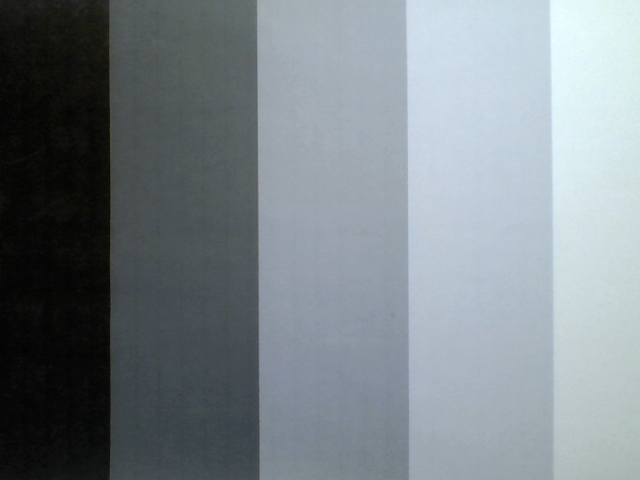
\includegraphics[scale=0.5]{media/grauwertkeil.png}
\captionof{figure}{Fig: Grauwertkeil, unbearbeitet}
\label{Fig:Grawertkeil}


\section{Auswertung}
\label{chap:VERSUCH_1_AUSWERTUNG}


\section{Interpretation}
\label{chap:VERSUCH_1_INTERPRETATION}


%
% CHAPTER Versuch 2
%

\chapter{Versuch 2}
\label{chap:VERSUCH_2}

\section{Fragestellung, Messprinzip, Aufbau, Messmittel}
\label{chap:VERSUCH_2_FRAGESTELLUNG}
\subsection*{Fragestellung}
Im 2 Versuch geht es darum durch die Aufnahme eines Dunkelbilds Pixel zu finden, die trotz kompletter Dunkelheit nicht den Wert 0(aus) zurück liefern.
\subsection*{Messprinzip}
Durch diesen Versuch werden die sogenannten Hot / Stuck Pixel erkannt(die Pixel die nicht 0 zurück liefern). Diese werden unter anderem durch das thermische Rauschen der Ausleseelektronik verursacht wird.
\subsection*{Aufbau}
Die Kamera wird vollständig verdunkelt zum Beispiel durch einen Aufkleber vor der Linse.
\subsection*{Messmittel}
Wie bei Versuch 1

\newpage
\section{Messwerte}
\label{chap:VERSUCH_2_MESSWERTE}
Es werden 10 Dunkelbild aufnahmen gemacht und in Grauwertbilder umgerechnet:
\linebreak
\begin{tabular}{ccccc}

\includegraphics[scale=0.1]{media/dunkelbilder/dunkelbild_0} & 
\includegraphics[scale=0.1]{media/dunkelbilder/dunkelbild_1} & 
\includegraphics[scale=0.1]{media/dunkelbilder/dunkelbild_2} & 
\includegraphics[scale=0.1]{media/dunkelbilder/dunkelbild_3} & 
\includegraphics[scale=0.1]{media/dunkelbilder/dunkelbild_4} \\ 

\includegraphics[scale=0.1]{media/dunkelbilder/dunkelbild_5} & 
\includegraphics[scale=0.1]{media/dunkelbilder/dunkelbild_6} & 
\includegraphics[scale=0.1]{media/dunkelbilder/dunkelbild_7} & 
\includegraphics[scale=0.1]{media/dunkelbilder/dunkelbild_8} & 

\includegraphics[scale=0.1]{media/dunkelbilder/dunkelbild_9} \\ 
\end{tabular} 


\section{Auswertung}
\label{chap:VERSUCH_2_AUSWERTUNG}
Aus den 10 Dunkelbild Aufnahmen wird dann der pixelweise Mittelwert berechnet und ein neues Dunkelbild erzeugt. Dies soll das thermische Ausleserauschen eliminieren und es bleibt nur noch der Offset jedes Pixels übrig:


\includegraphics[scale=0.4]{media/dunkelMean}

Auf dem ersten Blick sieht man nicht sehr viel. Allerdings wenn man das Dunkelbild Kontrast maximiert darstellt ergibt sich folgendes:

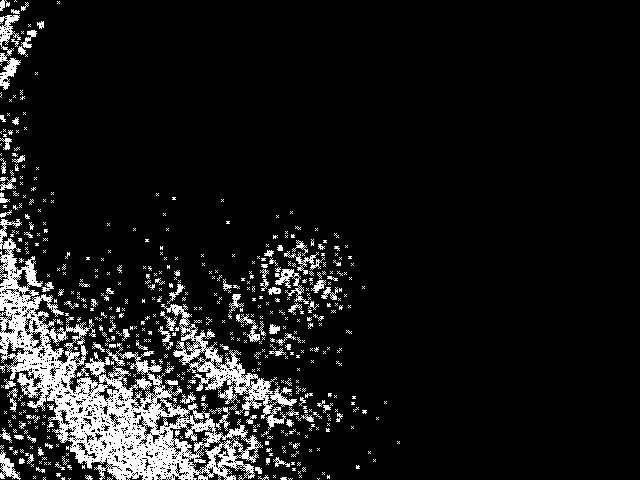
\includegraphics[scale=0.4]{media/dunkelContrastMax}

Jetzt wird jeder Pixel der aufgrund des thermischen Rauschens nicht den Wert 0 hat Kontrast maximiert dargestellt in weiß.

\section{Interpretation}
\label{chap:VERSUCH_2_INTERPRETATION}
Aus dem Kontrast maximierten Bild kann man sehr gut erkennen wie stark das Rauschen sein kann. Im Zusammenhang mit einer nicht sehr neuen Kamera die in diesem Fall verwendet wurde, ist das thermische Rauschen mit hoher Wahrscheinlichkeit viel stärker als bei neueren Kameras. 


%
% CHAPTER Versuch 3
%

\chapter{Versuch 3}
\label{chap:VERSUCH_3}

\section{Fragestellung, Messprinzip, Aufbau, Messmittel}
\label{chap:VERSUCH_3_FRAGESTELLUNG}

\subsection*{Fragesetellung}

Die Sensitivität von Kamerasensoren ist aufgrund von Fertigungstoleranzen nicht völlig gleich.
Zudem Kommt es durch das Objectiv der Kamera zu einer sogenannten Vignettierung, d.h. der Rand des Bildes ist dunkler als er sein sollte, weil das Licht ungleichmäßig verteilt wird.
Das beides führt dazu, das einige Pixel einen zu geringen Helligkeitswert aufweisen.
In diesen Versuch geht es darum diese Pixel zu finden und unsere Aufnahmen so zu kalibrieren das diese Pixel kein Problem mehr sind.

\subsection*{Messprinzip}
Wird eine Aufnahme von einen weißen Blatt Papier gemacht heben sich auf dem resultierenden Bild Schatten und zu dunkle Pixel hervor.
So kann man ermitteln welche Pixel einen zu dunklen Wert angeben.
Leider wird das Ergebnis durch starke Lichteinstrahlung und Schatten von außen verfälscht.
Daher ist es wichtig die Beleuchtung gleichmäßig zu halten, die Einflüsse äußeren Faktoren zu minimieren.

\subsection*{Aufbau}

\subsection{Messmittel}
\begin{itemize}
\item Webcame (Asus USB2.0 UVC HD Webcam)
\item weißes Blatt Papier
\item Metermaß
\end{itemize}


\section{Messwerte}
\label{chap:VERSUCH_3_MESSWERTE}

\begin{tabular}{|c|c|}
\hline 
\includegraphics[scale=0.25]{media/weisbilder/weisbild0.png}
 & 
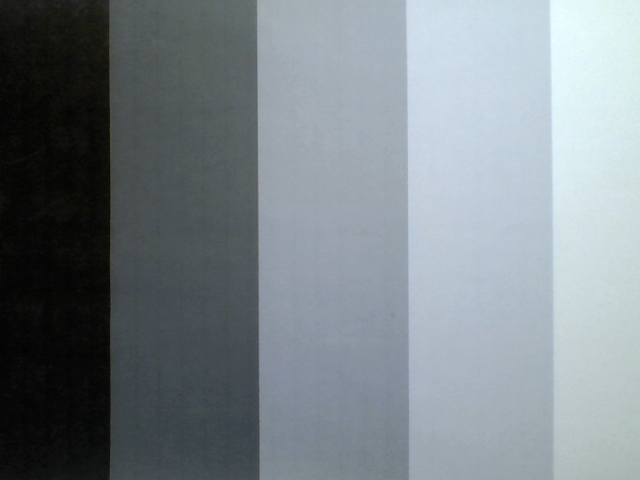
\includegraphics[scale=0.25]{media/grauwertkeil.png}
 \\ 
\hline 
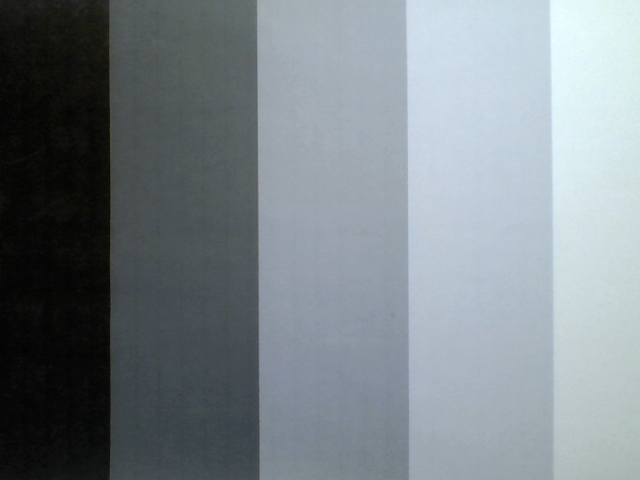
\includegraphics[scale=0.25]{media/grauwertkeil.png}
 & 
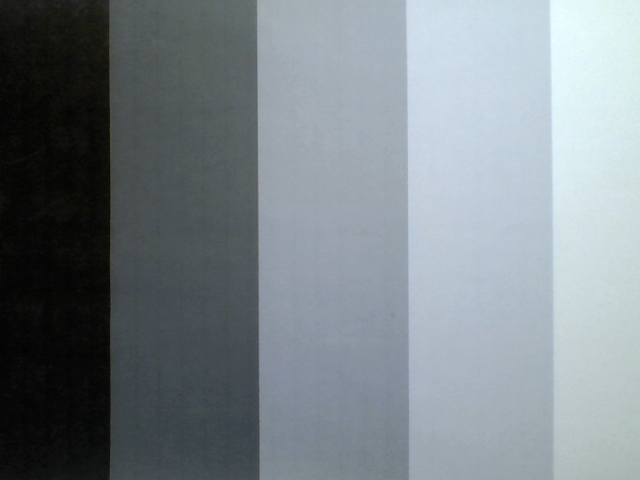
\includegraphics[scale=0.25]{media/grauwertkeil.png}
 \\ 
\hline 
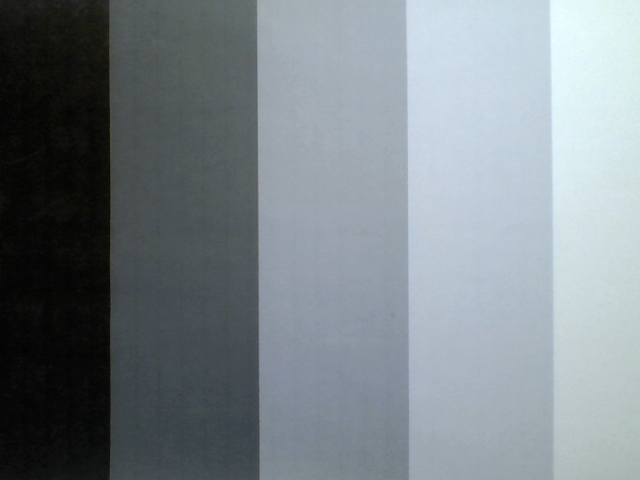
\includegraphics[scale=0.25]{media/grauwertkeil.png}
 & 
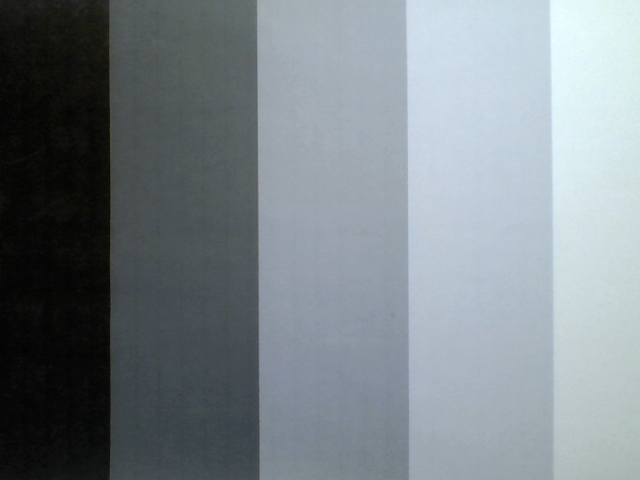
\includegraphics[scale=0.25]{media/grauwertkeil.png}
 \\ 
\hline 
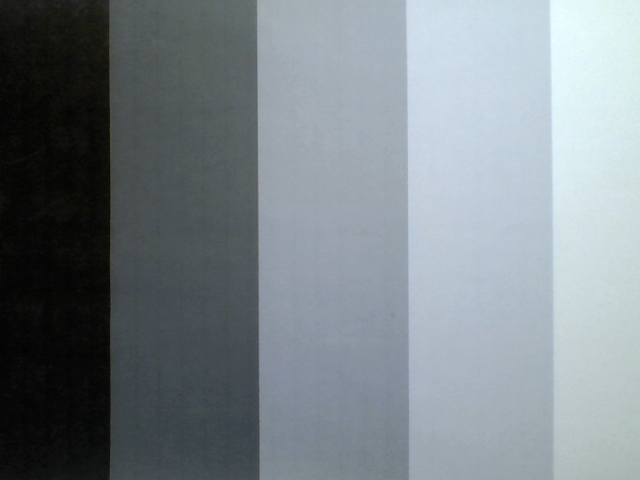
\includegraphics[scale=0.25]{media/grauwertkeil.png}
 & 
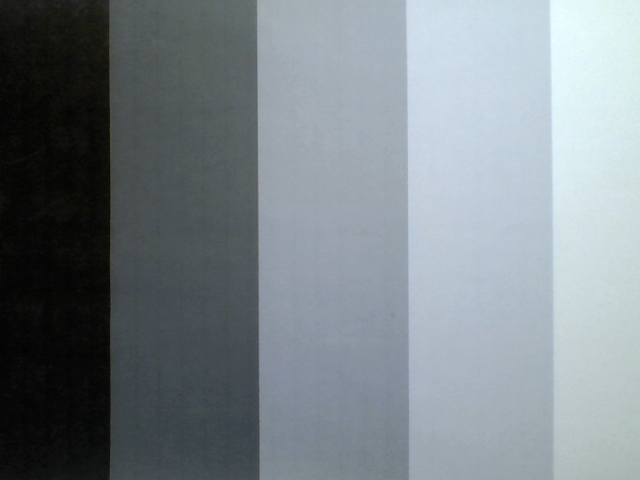
\includegraphics[scale=0.25]{media/grauwertkeil.png}
 \\ 
\hline 
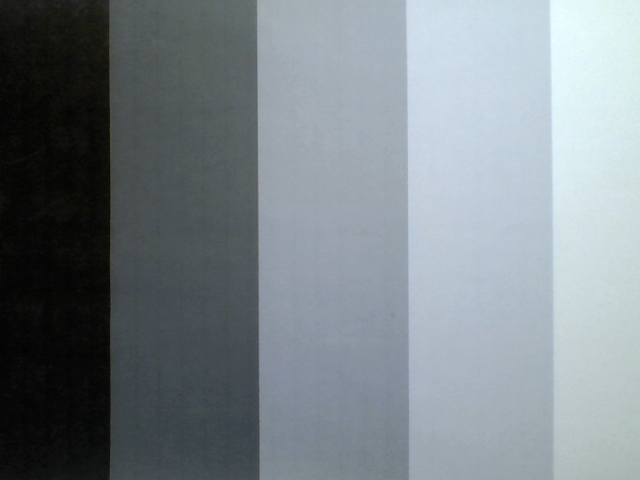
\includegraphics[scale=0.25]{media/grauwertkeil.png}
 & 
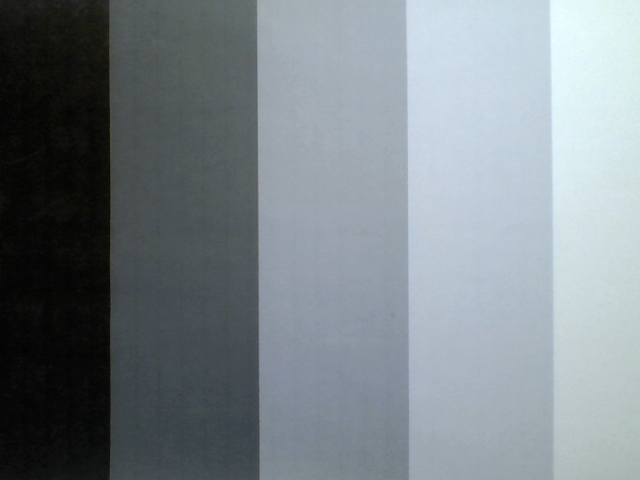
\includegraphics[scale=0.25]{media/grauwertkeil.png}
 \\ 
\hline 
\end{tabular} 

\section{Auswertung}
\label{chap:VERSUCH_3_AUSWERTUNG}

\section{Interpretation}
\label{chap:VERSUCH_3_INTERPRETATION}



%
% CHAPTER Versuch 4
%

\chapter{Versuch 4}
\label{chap:VERSUCH_4}

\section{Fragestellung, Messprinzip, Aufbau, Messmittel}
\label{chap:VERSUCH_4_FRAGESTELLUNG}

\subsection*{Fragestellung}
Aus den vorherigen Versuchen wurden verschiedene Berechnungen durchgeführt welche jetzt hier zusammen laufen. So geht es darum den aufgenommenen Grauwertkeil jetzt zu korrigieren mit den genannten Fehlern des Aufnahmesensors. 

\section{Auswertung}
\label{chap:VERSUCH_4_AUSWERTUNG}

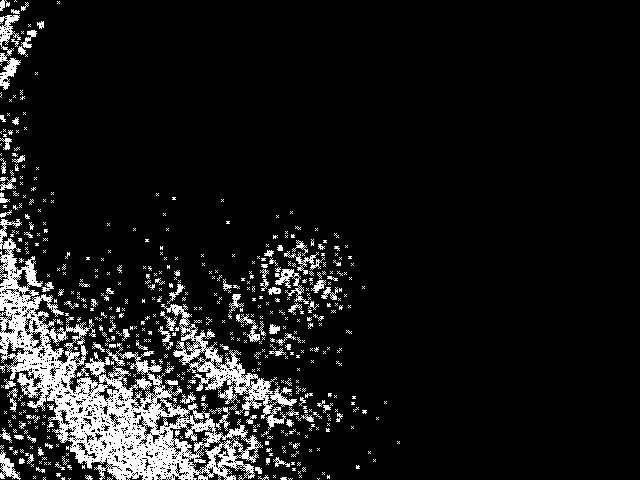
\includegraphics[scale=0.6]{media/dunkelContrastMax}

Wie man auf diesem Dunkelbild was Kontrast maximiert wurde gut erkennen kann, sind in der unteren linken Ecke nahezu alle Hot und Stuck Pixel(Alle Pixel die nicht den Wert 0 haben).

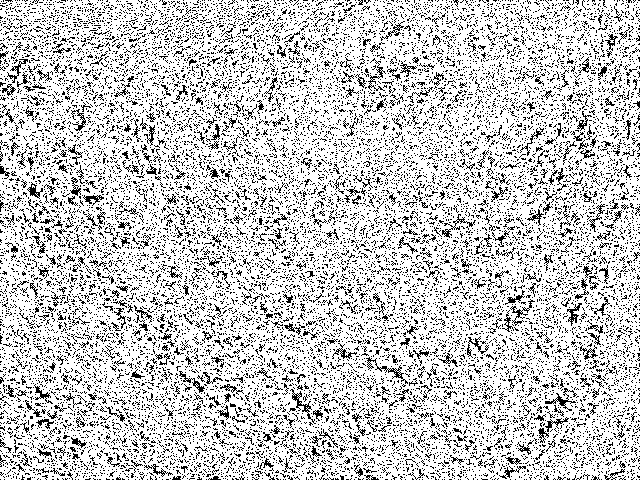
\includegraphics[scale=0.6]{media/weissContrastMax}

Hier ist das Gegenteil von dem Dunkelbild, ein Kontrast maximiertes Weißbild welches alle dead Pixels aufzeigt(Pixel die immer den wert 0 haben). Zusehen sind diese stärker in der unteren und oberen linken Ecke.

Aus diesen beiden Bildern wurde dann eine Kalibrierung durchgeführt mit dem ursprünglich erstelltem Bild von dem Grauwertkeil. Dabei wurde der Grauwertkeil minus dem Mittelwertbild des Dunkelbildes und anschließend minus dem normierten Mittelwertbild des Weißbildes gerechnet. Daraus folgen dann neue Werte des Grauwertkeils(Vorherige Werte siehe Tabelle Versuch 1):

\subsection*{Mittelwerte und Standardabweichung des Kalibrierten Grauwertkeilers}

\begin{tabular}{|c|c|c|}
\hline 
Graustufe & Mittelwert & Standardabweichung \\ 
\hline 
0 (schwarz) & 11.04 & 6.02 \\
\hline 
1 (dunkelgrau) & 81.14 & 8.1 \\ 
\hline 
2 (mittelgrau) & 150.12 & 8.85 \\ 
\hline 
3 (hellgrau) & 185.43 & 11.56 \\ 
\hline 
4 (weiß) & 214.03 & 14.37 \\ 
\hline 
\end{tabular} 
\captionof{table}{Tab:Grauwert2}
\newpage

\section{Interpretation}
\label{chap:VERSUCH_4_INTERPRETATION}
Wenn man den Grauwertkeil(vor und nach der Kalibrierung) jetzt miteinander vergleicht sieht man das sich fast überall die Standardabweichung verringert hat. Dies ist darauf zurück zu führen das wir aus den Grauwertkeil die Stuck, Hot und dead Pixels eliminiert haben durch die vorherige Versuche und Berechnungen.
Im allgemeinen folgt daraus ein einheitlicheres Bild ohne diese Störfaktoren und dies sieht dann folgender maßen aus:

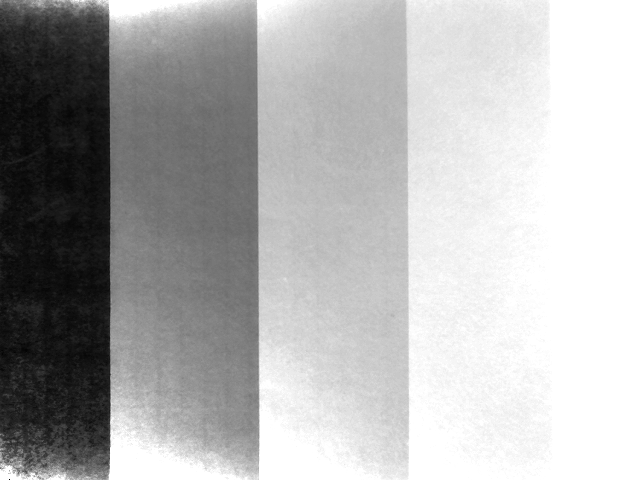
\includegraphics[scale=0.65]{media/grauWertKorrektur}


%
% CHAPTER Anhang
%
\renewcommand\thesection{A.\arabic{section}}
\renewcommand\thesubsection{\thesection.\arabic{subsection}}

\chapter*{Anhang}
\label{chap:APPENDIX}
\addcontentsline{toc}{chapter}{Anhang}
%\setcounter{chapter}{0}
\addtocounter{chapter}{1}
\setcounter{section}{0}

\section{Quellcode}
\label{chap:APPENDIX_SOURCECODE}

\subsection{Quellcode Versuch 1}
\label{chap:APPENDIX_SOURCECODE_V1}

\subsection{Quellcode Versuch 2}
\label{chap:APPENDIX_SOURCECODE_V2}

\subsection{Quellcode Versuch 3}
\label{chap:APPENDIX_SOURCECODE_V3}

\subsection{Quellcode Versuch 4}
\label{chap:APPENDIX_SOURCECODE_V4}


\section{Messergebnisse}
\label{chap:APPENDIX_MEASUREMENT_SOURCE}

%
% Literaturverzeichnis
%
%
% Literaturverzeichnis
%
\phantomsection
\addcontentsline{toc}{chapter}{Literaturverzeichnis}
\bibliography{../references}
\newpage

\end{document}
%------------------------------------
% ╔═╗╔╗╔╔╦╗  ╔╦╗╔═╗╔═╗╦ ╦╔╦╗╔═╗╔╗╔╔╦╗
% ║╣ ║║║ ║║   ║║║ ║║  ║ ║║║║║╣ ║║║ ║
% ╚═╝╝╚╝═╩╝  ═╩╝╚═╝╚═╝╚═╝╩ ╩╚═╝╝╚╝ ╩
%------------------------------------